\documentclass[aspectratio=169]{beamer}

\usetheme{strath}

\usepackage[UKenglish]{babel}
\usepackage[nodayofweek]{datetime}
\usepackage{listings}

\graphicspath{{img/}}

\title[Sample presentation]{Sample Beamer presentation}
\author[Author]{Author Name}
\institute{University of Strathclyde}
\date[\dmyydate\today]{\longdate\today}

\begin{document}

\frame{\titlepage}

\begin{frame}[fragile]{Sample frame title}
	For main/corporate theme, call \verb|\usetheme{strath}|
	\vspace{0.6cm}
	\begin{columns}
		\begin{column}{0.47\textwidth}
			\begin{enumerate}
				\item A
				\item Numbered
				\item List
			\end{enumerate}
		\end{column}
		\begin{column}{0.47\textwidth}
			\begin{itemize}
				\item Some
				\item Bullet
				\item Points
			\end{itemize}
		\end{column}
	\end{columns}
\end{frame}

\begin{frame}[fragile]{Engineering theme}
	\begin{columns}
		\begin{column}{0.5\textwidth}
			\tcbincludegraphics[width=\textwidth]{eng1.png}
		\end{column}
		\begin{column}{0.5\textwidth}
			\tcbincludegraphics[width=\textwidth]{eng2.png}
		\end{column}
	\end{columns}
	\vspace{0.6cm}
	\centering
	\verb|\usetheme[eng]{strath}|
\end{frame}

\begin{frame}[fragile]{Science theme}
	\begin{columns}
		\begin{column}{0.5\textwidth}
			\tcbincludegraphics[width=\textwidth]{sci1.png}
		\end{column}
		\begin{column}{0.5\textwidth}
			\tcbincludegraphics[width=\textwidth]{sci2.png}
		\end{column}
	\end{columns}
	\vspace{0.6cm}
	\centering
	\verb|\usetheme[sci]{strath}|
\end{frame}

\begin{frame}[fragile]{HaSS theme}
	\begin{columns}
		\begin{column}{0.5\textwidth}
			\tcbincludegraphics[width=\textwidth]{hass1.png}
		\end{column}
		\begin{column}{0.5\textwidth}
			\tcbincludegraphics[width=\textwidth]{hass2.png}
		\end{column}
	\end{columns}
	\vspace{0.6cm}
	\centering
	\verb|\usetheme[hass]{strath}|
\end{frame}

\begin{frame}[fragile]{Business School theme}
	\begin{columns}
		\begin{column}{0.5\textwidth}
			\tcbincludegraphics[width=\textwidth]{sbs1.png}
		\end{column}
		\begin{column}{0.5\textwidth}
			\tcbincludegraphics[width=\textwidth]{sbs2.png}
		\end{column}
	\end{columns}
	\vspace{0.6cm}
	\centering
	\verb|\usetheme[sbs]{strath}|
\end{frame}

\begin{frame}{Frame title}{Frames can have subtitles}
	\begin{block}{Block}
		Something in a regular block
	\end{block}
	\begin{exampleblock}{Example block}
		Something in an example block
	\end{exampleblock}
	\begin{alertblock}{Alert block}
		Something in an alert block
	\end{alertblock}
\end{frame}

\begin{frame}{Aspect ratios}{Branding side bar is removed for narrow aspect ratios}
	\begin{columns}
		\begin{column}{0.5\textwidth}
			\begin{block}{4:3 aspect ratio}
				\centering
				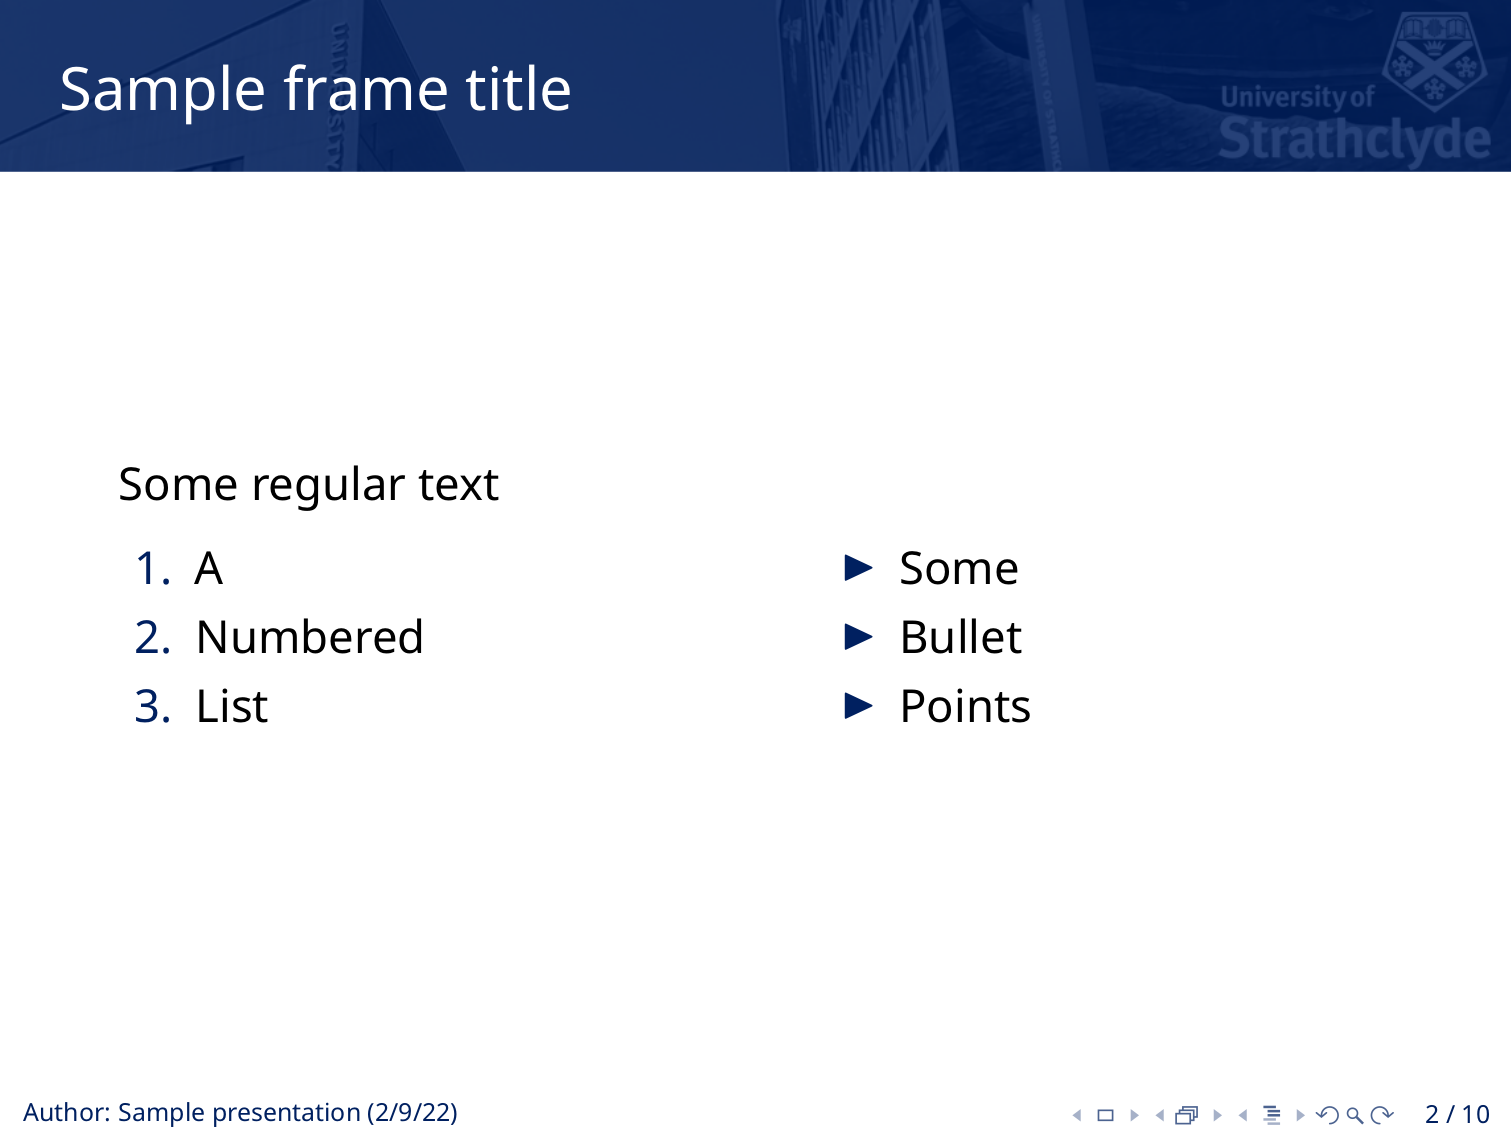
\includegraphics[height=3cm]{ar43.png}
			\end{block}
		\end{column}
		\begin{column}{0.5\textwidth}
			\begin{block}{16:9 aspect ratio}
				\centering
				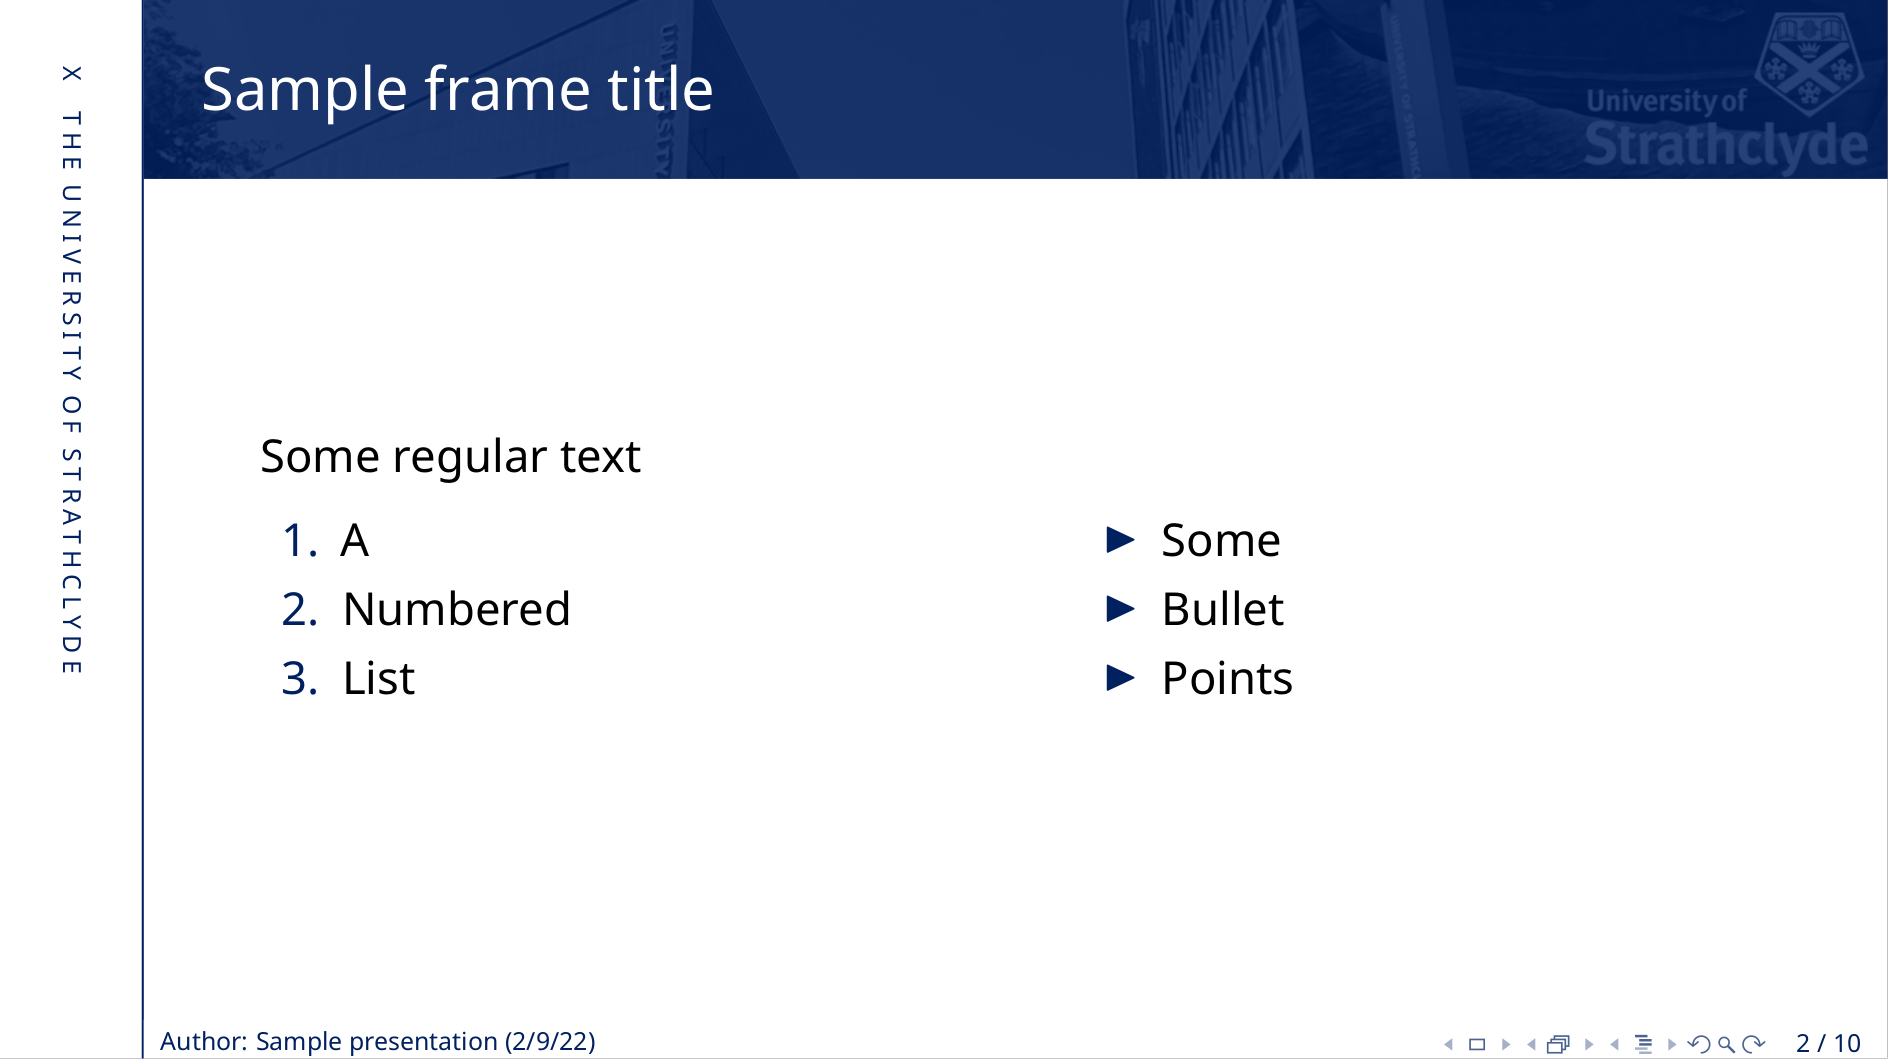
\includegraphics[height=3cm]{ar169.png}
			\end{block}
		\end{column}
	\end{columns}
\end{frame}

\begin{frame}[fragile]{\texttt{\textbackslash{}ifratio} command}
	\begin{block}{}
		Helper command for changing layout based on aspect ratio
	\end{block}
	\begin{exampleblock}{Example}
		\begin{lstlisting}[language=TeX, gobble=3, tabsize=1]
			\ifratio{43}{
			  % Code for 4:3 ratio
			}{
			  % Code for any other ratio
			}
		\end{lstlisting}
	\end{exampleblock}
\end{frame}

\begin{frame}[fragile]{\texttt{\textbackslash{}fillgraphics} command}
	\fillgraphics[0.33]{strath.png}
	\begin{columns}
		\begin{column}{0.33\textwidth}
		\end{column}
		\begin{column}{0.65\textwidth}
			\begin{block}{}
				Helper command to stretch and clip an image in the background to make it fill a portion of the frame
			\end{block}
			\begin{block}{}
				First option specifies width relative to viewport (defaults to 1 for full width)
			\end{block}
			\begin{exampleblock}{Code}\small
				\verb|\fillgraphics[0.33]{strath.png}|
			\end{exampleblock}
		\end{column}
	\end{columns}
\end{frame}

\begin{frame}[fragile]{\texttt{\textbackslash{}fillgraphics} command}
	\fillgraphics[0.25][1]{strath.png}
	\begin{columns}
		\begin{column}{0.72\textwidth}
			\begin{block}{}
				Second option specifies horizontal position\\
				(defaults to 0 for left-aligned)
			\end{block}
			\begin{exampleblock}{Code}
				\texttt{\textbackslash{}fillgraphics[0.25][1]{strath.png}}
			\end{exampleblock}
			\begin{alertblock}{Reminder}
				Listings and verbatim environments in beamer require the frame to have the \verb|fragile| option
			\end{alertblock}
		\end{column}
		\begin{column}{0.25\textwidth}
		\end{column}
	\end{columns}
\end{frame}

\begingroup\setbeamertemplate{footline}{}
\begin{frame}[fragile]
	\fillgraphics[1][0][0pt]{strath.png}
	\begin{block}{}
		Third option specifies top trim amount\\
		(defaults to height of frame title banner)
	\end{block}
	\begin{exampleblock}{Code}
		\verb|\fillgraphics[1][0][0pt]{strath.png}|
	\end{exampleblock}
	\begin{alertblock}{To remove footlines}
		\begin{lstlisting}[language=TeX, gobble=3, tabsize=1]
			\begingroup\setbeamertemplate{footline}{}
			  % Frames without footlines
			\endgroup
		\end{lstlisting}
	\end{alertblock}
\end{frame}
\endgroup

\end{document}
